% Created 2016-08-17 Wed 14:38
\documentclass[tikz]{standalone}

\usepackage[utf8]{inputenc}
\usepackage[T1]{fontenc}

\usepackage{circledsteps}

\RequirePackage{xcolor}

%% HPI color definitions according to the design manual
% These do not exactly match the RGB values used in the Powerpoint slide master due to unknown reasons
\definecolor{hpiyellow}{RGB}{246,168,0}
\definecolor{hpiorange}{RGB}{221,97,8}
\definecolor{hpired}{RGB}{177,6,58}
\definecolor{hpigray}{RGB}{90,96,101}
\definecolor{hpiblue}{RGB}{0,122,158}


\renewcommand{\sfdefault}{neosans}
% Different font weights for neosans
\newcommand{\textl}[1]{{\fontseries{l}\selectfont #1}} % light
\newcommand{\textm}[1]{{\fontseries{m}\selectfont #1}} % medium, same as default weight
\newcommand{\textsb}[1]{{\fontseries{sb}\selectfont #1}} % semibold
\newcommand{\textmb}[1]{{\fontseries{mb}\selectfont #1}} % bold, same as \textbf
\newcommand{\texteb}[1]{{\fontseries{eb}\selectfont #1}} % extra bold
\newcommand{\textub}[1]{{\fontseries{ub}\selectfont #1}} % ultra bold

\tikzset{every picture/.style={/utils/exec={\sffamily}}}
\tikzset{flipflop RSflanke/.style={
  flipflop,
  flipflop def={t1=S, t2=C, c2=1, t3=R, t6=Q, t4={\ctikztextnot{Q}}}
}}


\tikzset{
  mechanicalSwitch/.pic={
    \coordinate (-inUp) at (135:2); 
    \coordinate (-inDown) at (235:2);
    \coordinate (-out) at (2,0);
    \coordinate (-center) at (0,0);
    
    \draw (0,0) circle [radius = 2cm];
    \draw [fill=gray!20] (0,0) circle [radius = 0.2cm];

    \draw (0, 0) -- (2, 0);
    \draw (135:.8) -- (135:2); 
    \draw (225:.8) -- (225:2); 

    \draw [fill=gray!20] (2, 0) circle [radius=0.05cm]; 
    \draw [fill=gray!20] (135:2) circle [radius=0.05cm]; 
    \draw [fill=gray!20] (225:2) circle [radius=0.05cm]; 

    
    \draw [thick] (0,0) -- (175:1.5); 

    \draw [dashed, <->, domain=135:225] plot ({cos(\x)}, {sin(\x)}); 
  },
  mechanicalSwitchClosed/.pic={
    \coordinate (-inUp) at (135:2); 
    \coordinate (-inDown) at (255:2);
    \coordinate (-out) at (2,0);
    \coordinate (-center) at (0,0);
    \draw (0,0) circle [radius = 2cm];
    \draw [fill=gray!20] (0,0) circle [radius = 0.2cm];

    \draw (0, 0) -- (2, 0);
    \draw (135:.8) -- (135:2); 
    \draw (225:.8) -- (225:2); 

    \draw [fill=gray!20] (2, 0) circle [radius=0.05cm]; 
    \draw [fill=gray!20] (135:2) circle [radius=0.05cm]; 
    \draw [fill=gray!20] (225:2) circle [radius=0.05cm]; 

    
    \draw [thick] (0,0) -- (135:2); 

    \draw [dashed, <->, domain=135:225] plot ({cos(\x)}, {sin(\x)}); 
  }
}


\usetikzlibrary{calc}
\usetikzlibrary{positioning}


\usepackage{../../templates/moeptikz}
\usepackage{booktabs}

\usetikzlibrary{chains,backgrounds,fit,patterns}

% TODO: This should be turned into a proper tikz decoration :-/ 
\newcommand{\variableLength}[1]{
  \foreach \o in {north,south} {
  \draw[line width=1.6pt, -] 
  ($(#1.\o)+(0pt,4pt)$) .. controls + (2pt,-2pt) and + (-2pt,2pt) .. ++(0pt,-8pt);
  \draw[white, line width=1pt, solid, -]
  ($(#1.\o)+(0pt,4.1pt)$) .. controls + (2pt,-2pt) and + (-2pt,2pt) .. ++(0pt,-8.2pt);
  }
}



\begin{document}

\begin{tikzpicture}
  \label{page:inter:happy_ether}
  \node [server] (server) {}; 
  \node [client, right=of server] (client) {}; 

  \draw [hpiyellow, very thick] ($(server)+(-1,-1)$)  -- ($(client)+(1,-1)$) ; 

  \draw [hpiyellow, thick] (server) -- ++(0, -1) node [circle, fill=hpiyellow, scale=0.5] {};
  \draw [hpiyellow, thick] (client) -- ++(0, -1) node [circle, fill=hpiyellow, scale=0.5] {}; 
\end{tikzpicture}


\begin{tikzpicture}
  \label{page:inter:sad_ether}

  \draw [hpiyellow, very thick] (1,0) -- (14,0); 
  
  \foreach \i in {1,...,6} {
    
    \node [server] (server\i) at (2*\i,-1) {};
    \node [client] (client\i) at (1+2*\i,1) {};

    \draw [hpiyellow, thick] (server\i) -- (2*\i, 0) node [circle, fill=hpiyellow, scale=0.5] {};
    \draw [hpiyellow, thick] (client\i) --(1+2*\i, 0) node [circle, fill=hpiyellow, scale=0.5] {}; 
    
  }
  

\end{tikzpicture}


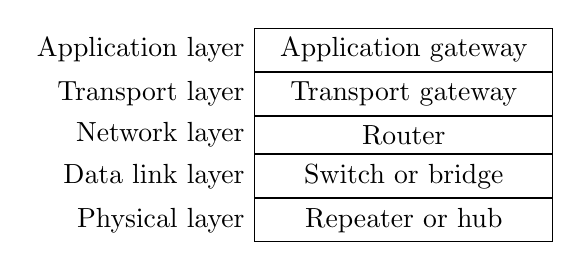
\begin{tikzpicture}[start chain=1 going below, node distance=0pt]
  \label{page:inter:gateway_names}

  \foreach \layer/\inter in {Application/Application gateway,Transport/Transport gateway,Network/Router,Data link/Switch or bridge,Physical/Repeater or hub} {
    \node [on chain=1, draw, minimum width=25ex, label=left:\layer\ layer] {\inter}; 
  }

  
\end{tikzpicture}


\begin{tikzpicture}
  \label{page:inter:repeater}

  \node [draw] (repeater) {Repeater};

  \draw (repeater) edge  node [midway, above] {Signal in} ++(-4, 0); 
  \draw (repeater) edge node [midway, above] {Signal out} ++(+4, 0) ; 
  
\end{tikzpicture}


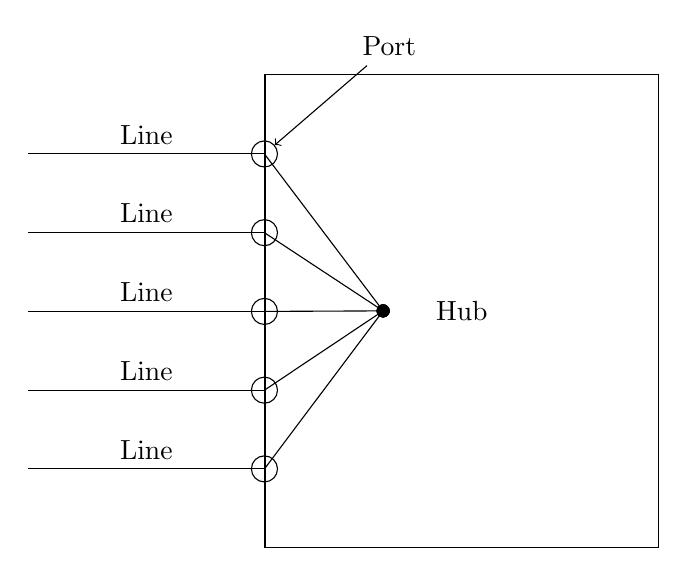
\begin{tikzpicture}
  \label{page:inter:hub}

  \node [draw, minimum height=6cm, minimum width=5cm] (hub) {Hub};

  \foreach \i in {1,...,5} {
    \node [circle, draw] at ($(hub.south west)+(0, \i)$)  (port\i) {}; 
    \draw ($(hub.center)+(-1, 0)$) node [circle, fill, scale=0.5] {} --   ($(hub.south west)+(0,\i)$) edge  node [midway, above] {Line} ++(-3, 0);

  }

  \node [above right=of port5] (portlabel) {Port};
  \draw [->] (portlabel) -- (port5); 
\end{tikzpicture}

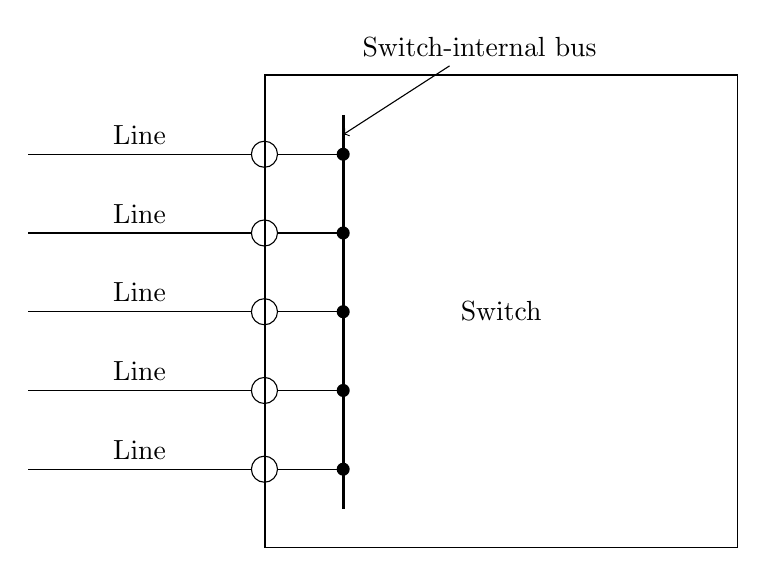
\begin{tikzpicture}
  \label{page_inter:switch:busbased}

  
  \node [draw, minimum height=6cm, minimum width=6cm] (switch) {Switch};

  \foreach \i in {1,...,5} {
    \node [circle, draw] at ($(switch.south west)+(0, \i)$)  (port\i) {}; 
    \draw (port\i) --  ++(1,0) node [circle, fill, scale=0.5] {};
    \draw (port\i) --  node [midway, above] {Line} ++(-3, 0);

  }

  \draw  [very thick] ($(port5)+(1,0.5)$) -- ($(port1) +(1,-0.5)$) ;
  \node [above right=of port5] (buslabel) {Switch-internal bus};
  \draw [->] (buslabel) -- ($(port5) + (1,0.25)$); 

\end{tikzpicture}

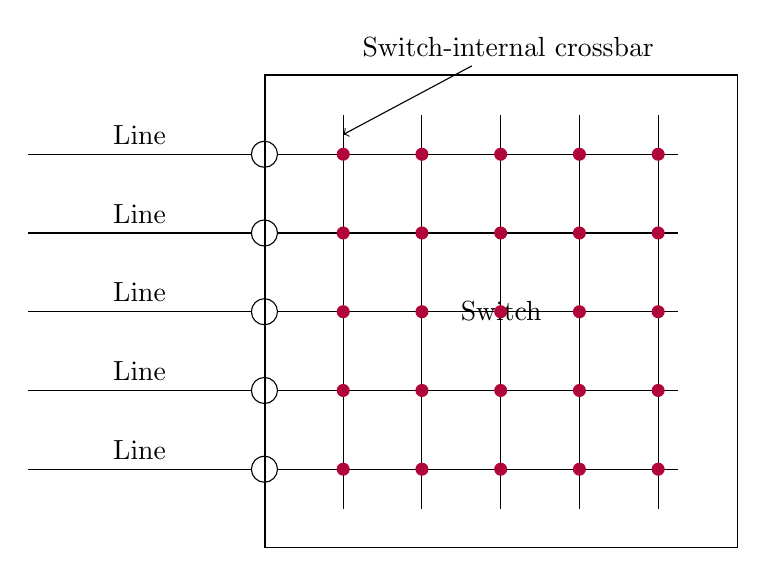
\begin{tikzpicture}
  \label{page_inter:switch:crossbar_based}

  
  \node [draw, minimum height=6cm, minimum width=6cm] (switch) {Switch};

  \foreach \i in {1,...,5} {
    \node [circle, draw] at ($(switch.south west)+(0, \i)$)  (port\i) {}; 
    \draw (port\i) --  ++(5.25,0); %  node [circle, fill, scale=0.5] {};
    \draw (port\i) --  node [midway, above] {Line} ++(-3, 0);
  }

  \foreach \i in {1,...,5} {
    \draw ($(port5) + (\i,0.5)$) -- ($(port1) +(\i,-0.5)$); 
    \foreach \j in {1,...,5} {
      \node [hpired, circle, fill, scale=0.5] at ($(port5) + (\i,1-\j)$) {};
    }
  }
  
%   \draw  [very thick] ($(port5)+(1,0.5)$) -- ($(port1) +(1,-0.5)$) ;
  \node [above right=of port5] (buslabel) {Switch-internal crossbar};
  \draw [->] (buslabel) -- ($(port5) + (1,0.25)$); 

\end{tikzpicture}

\begin{tikzpicture}
  \label{page:inter:bridge}

  \node [switch] at (0,0) (bridge) {Bridge}; 
  \foreach \i in {1,...,5} {
    \node [client] at (-4, 3-\i) (cl\i) {};
    \draw (cl\i) -- (bridge); 
  }
  \foreach \i in {1,...,3} {
    \node [server] at (+4, 2-\i) (srv\i) {}; 
    \draw (srv\i) -- (bridge); 
  }

  \begin{scope}[on background layer]
    \node [fill=hpiyellow!10, fit=(cl1)(cl2)(cl3)(cl4)(cl5)(bridge.west)] {};
    \node [fill=hpiblue!10, fit=(srv1)(srv2)(srv3)(bridge.east)] {};
  \end{scope}
  
\end{tikzpicture}

\begin{tikzpicture}
  \label{page:inter:bridge_switch}

  \node [switch] at (0,0) (bridge) {Bridge};
  \node [switch] at (-2,0) (switch1) {Switch 1};
  \node [switch] at (2,0) (switch2) {Switch 2};

  \draw [thick] (switch1) -- (bridge) -- (switch2); 
  
  \foreach \i in {1,...,5} {
    \node [client] at (-4, 3-\i) (cl\i) {};
    \draw (cl\i) -- (switch1); 
  }
  \foreach \i in {1,...,3} {
    \node [server] at (+4, 2-\i) (srv\i) {}; 
    \draw (srv\i) -- (switch2); 
  }
  
  \begin{scope}[on background layer]
    \node [fill=hpiyellow!10, fit=(cl1)(cl2)(cl3)(cl4)(cl5)(bridge.west)(switch1)] {};
    \node [fill=hpiblue!10, fit=(srv1)(srv2)(srv3)(bridge.east)(switch2)] {};
  \end{scope}
\end{tikzpicture}


\begin{tikzpicture}
  \label{page:inter:two_switches}

  \node [switch] at (-2,0) (switch1) {Switch 1};
  \node [switch] at (2,0) (switch2) {Switch 2};

  \draw [thick] (switch1) -- (switch2); 
  
  \foreach \i in {1,...,5} {
    \node [client] at (-4, 3-\i) (cl\i) {};
    \draw (cl\i) -- (switch1); 
  }
  \foreach \i in {1,...,3} {
    \node [server] at (+4, 2-\i) (srv\i) {}; 
    \draw (srv\i) -- (switch2); 
  }
  
  \begin{scope}[on background layer]
    \node [fill=hpiyellow!10, fit=(cl1)(cl2)(cl3)(cl4)(cl5)(switch1)(srv1)(srv2)(srv3)(switch2)] {};
  \end{scope}
\end{tikzpicture}


\begin{tikzpicture}
  \label{page:inter:backward:simple:before}

  \node [client] at (-5,0) (cl) {}; 
  \node [switch] at (0,0) (sw) {}; 
  \node [client] at (5,0) (srv) {}; 

  \draw [very thick] (cl) -- (sw) -- (srv);

  \foreach \l/\s in {a:b/cl.east,c:d/sw.west,e:f/sw.east,g:h/srv.west} {
    \node [above=of \s] {\l}; 
  }

  \node [below=0.5 of sw, align=center] {Forwarding \\table:\\
    \begin{tabular}{ll}
      \toprule
      Dest. & Out \\
      & port \\
      \midrule
      -- & -- \\
      \bottomrule 
    \end{tabular}
  }; 
  
  \node [draw, above left=0.3 of sw.west] (pkt) {From: a:b, to: g:h};
  \draw [->, very thick] (pkt.east) -- ++(0.5,0); 
  
\end{tikzpicture}

\begin{tikzpicture}
  \label{page:inter:backward:simple:after}

  \node [client] at (-5,0) (cl) {}; 
  \node [switch] at (0,0) (sw) {}; 
  \node [client] at (5,0) (srv) {}; 

  \draw [very thick] (cl) -- (sw) -- (srv);

  \foreach \l/\s in {a:b/cl.east,c:d/sw.west,e:f/sw.east,g:h/srv.west} {
    \node [above=of \s] {\l}; 
  }

  \node [below=0.5 of sw, align=center] {Forwarding \\table:\\
    \begin{tabular}{ll}
      \toprule
      Dest. & Out \\
      & port \\
      \midrule
      a:b & c:d \\
      \bottomrule 
    \end{tabular}
  }; 
  
  \node [draw, above right=0.3 of sw.east] (pkt) {From: a:b, to: g:h};
  \draw [->, very thick] (pkt.east) -- ++(0.5,0); 
  
\end{tikzpicture}


\begin{tikzpicture}
  \label{page:inter:backward:two_switches:before}

  \node [client] at (-5,0) (cl) {}; 
  \node [switch] at (0,0) (sw1) {}; 
  \node [switch] at (5,0) (sw2) {}; 
  \node [client] at (10,0) (srv) {}; 

  \draw [very thick] (cl) -- (sw1) --(sw2) -- (srv);

  \foreach \l/\s in {a:b/cl.east,c:d/sw1.west,e:f/sw1.east,g:h/srv.west,k:l/sw2.west,m:n/sw2.east} {
    \node [above=of \s] {\l}; 
  }

  \node [below=0.5 of sw1, align=center] {Forwarding \\table:\\
    \begin{tabular}{ll}
      \toprule
      Dest. & Out \\
      & port \\
      \midrule
      -- & -- \\
      \bottomrule 
    \end{tabular}
  }; 

  \node [below=0.5 of sw2, align=center] {Forwarding \\table:\\
    \begin{tabular}{ll}
      \toprule
      Dest. & Out \\
      & port \\
      \midrule
      -- & -- \\
      \bottomrule 
    \end{tabular}
  }; 

  
  \node [draw, above left=0.3 of sw1.west] (pkt) {From: a:b, to: g:h};
  \draw [->, very thick] (pkt.east) -- ++(0.5,0); 
  
\end{tikzpicture}


\begin{tikzpicture}
  \label{page:inter:backward:two_switches:step1}

  \node [client] at (-5,0) (cl) {}; 
  \node [switch] at (0,0) (sw1) {}; 
  \node [switch] at (5,0) (sw2) {}; 
  \node [client] at (10,0) (srv) {}; 

  \draw [very thick] (cl) -- (sw1) --(sw2) -- (srv);

  \foreach \l/\s in {a:b/cl.east,c:d/sw1.west,e:f/sw1.east,g:h/srv.west,k:l/sw2.west,m:n/sw2.east} {
    \node [above=of \s] {\l}; 
  }

  \node [below=0.5 of sw1, align=center] {Forwarding \\table:\\
    \begin{tabular}{ll}
      \toprule
      Dest. & Out \\
      & port \\
      \midrule
      a:b & c:d \\
      \bottomrule 
    \end{tabular}
  }; 

  \node [below=0.5 of sw2, align=center] {Forwarding \\table:\\
    \begin{tabular}{ll}
      \toprule
      Dest. & Out \\
      & port \\
      \midrule
      -- & -- \\
      \bottomrule 
    \end{tabular}
  }; 

  
  \node [draw, above left=0.3 of sw2.west] (pkt) {From: a:b, to: g:h};
  \draw [->, very thick] (pkt.east) -- ++(0.5,0); 
  
\end{tikzpicture}

\begin{tikzpicture}
  \label{page:inter:backward:two_switches:step2}

  \node [client] at (-5,0) (cl) {}; 
  \node [switch] at (0,0) (sw1) {}; 
  \node [switch] at (5,0) (sw2) {}; 
  \node [client] at (10,0) (srv) {}; 

  \draw [very thick] (cl) -- (sw1) --(sw2) -- (srv);

  \foreach \l/\s in {a:b/cl.east,c:d/sw1.west,e:f/sw1.east,g:h/srv.west,k:l/sw2.west,m:n/sw2.east} {
    \node [above=of \s] {\l}; 
  }

  \node [below=0.5 of sw1, align=center] {Forwarding \\table:\\
    \begin{tabular}{ll}
      \toprule
      Dest. & Out \\
      & port \\
      \midrule
      a:b & c:d \\
      \bottomrule 
    \end{tabular}
  }; 

  \node [below=0.5 of sw2, align=center] {Forwarding \\table:\\
    \begin{tabular}{ll}
      \toprule
      Dest. & Out \\
      & port \\
      \midrule
      a:b & k:l \\
      \bottomrule 
    \end{tabular}
  }; 

  
  \node [draw, above right=0.3 of sw2.east] (pkt) {From: a:b, to: g:h};
  \draw [->, very thick] (pkt.east) -- ++(0.5,0); 
  
\end{tikzpicture}

\begin{tikzpicture}
  \label{page:inter:backward:two_switches:step3}

  \node [client] at (-5,0) (cl) {}; 
  \node [switch] at (0,0) (sw1) {}; 
  \node [switch] at (5,0) (sw2) {}; 
  \node [client] at (10,0) (srv) {}; 

  \draw [very thick] (cl) -- (sw1) --(sw2) -- (srv);

  \foreach \l/\s in {a:b/cl.east,c:d/sw1.west,e:f/sw1.east,g:h/srv.west,k:l/sw2.west,m:n/sw2.east} {
    \node [above=of \s] {\l}; 
  }

  \node [below=0.5 of sw1, align=center] {Forwarding \\table:\\
    \begin{tabular}{ll}
      \toprule
      Dest. & Out \\
      & port \\
      \midrule
      a:b & c:d \\
      \bottomrule 
    \end{tabular}
  }; 

  \node [below=0.5 of sw2, align=center] {Forwarding \\table:\\
    \begin{tabular}{ll}
      \toprule
      Dest. & Out \\
      & port \\
      \midrule
      a:b & k:l \\
      g:h & m:n \\
      \bottomrule 
    \end{tabular}
  }; 

  
  \node [draw, above left=0.3 of sw2.west] (pkt) {From: g:h, to: a:b};
  \draw [->, very thick] (pkt.west) -- ++(-0.5,0); 
  
\end{tikzpicture}

\begin{tikzpicture}
  \label{page:inter:backward:two_switches:step4}

  \node [client] at (-5,0) (cl) {}; 
  \node [switch] at (0,0) (sw1) {}; 
  \node [switch] at (5,0) (sw2) {}; 
  \node [client] at (10,0) (srv) {}; 

  \draw [very thick] (cl) -- (sw1) --(sw2) -- (srv);

  \foreach \l/\s in {a:b/cl.east,c:d/sw1.west,e:f/sw1.east,g:h/srv.west,k:l/sw2.west,m:n/sw2.east} {
    \node [above=of \s] {\l}; 
  }

  \node [below=0.5 of sw1, align=center] {Forwarding \\table:\\
    \begin{tabular}{ll}
      \toprule
      Dest. & Out \\
      & port \\
      \midrule
      a:b & c:d \\
      g:h & e:f \\
      \bottomrule 
    \end{tabular}
  }; 

  \node [below=0.5 of sw2, align=center] {Forwarding \\table:\\
    \begin{tabular}{ll}
      \toprule
      Dest. & Out \\
      & port \\
      \midrule
      a:b & k:l \\
      g:h & m:n \\
      \bottomrule 
    \end{tabular}
  }; 

  
  \node [draw, above left=0.3 of sw1.west] (pkt) {From: g:h, to: a:b};
  \draw [->, very thick] (pkt.west) -- ++(-0.5,0); 
  
\end{tikzpicture}


\begin{tikzpicture}
  \label{page:inter:complex:backwardlearning}

  \node [draw] (hub) {Hub};

  \node [above left= of hub, client] (cl1a) {Cl 1a}; 
  \node [below left= of hub, client] (cl1b) {Cl 1b};

  \node [switch, right=of hub] (switch)  {Bridge 1};

  \node [switch, right=4 of switch] (bridge) {Bridge 2};

  \node [switch, above right=of bridge] (sw2) {Switch 1}; 
  \node [switch, below right=of bridge] (sw3) {Switch 2};

  \node [client, above right=of sw2] (cl2a) {Cl 2a}; 
  \node [client, right=of cl2a] (cl2b) {Cl 2b}; 
  \node [client, right=of cl2b] (cl2c) {Cl 2c};


  \node [server, below right=of sw3] (srv3a) {Server 1}; 
  \node [server, right=of srv3a] (srv3b) {Server 2};
  \node [below=0.5 of srv3a] {}; % bug fix 

  \node [client, above right=of switch] (oldclient) {Old client}; 
  % links:

  \draw (cl1a) -- (hub) edge (cl1b) -- (switch);
  \draw [very thick, hpiyellow] (switch) -- (bridge); 
  \draw [very thick, hpiyellow] (switch -| oldclient) -- (oldclient);

  \draw (sw2) |- (bridge) -| (sw3);

  \foreach \i in {a,b,c} {\draw (sw2) -| (cl2\i);}
  \foreach \i in {a,b} {\draw (sw3) -| (srv3\i);}
  
  
\end{tikzpicture}

\begin{tikzpicture}

  \node [switch] at (2, 1)(sw1) {Switch 1};
  \node [right=0.1 of sw1.south] {c:d}; 
  \node [right=0.1cm of sw1.north] {e:f}; 
  \node [switch] at (6, 1)(sw2) {Switch 2}; 
  \node [left=0.1 of sw2.south] {g:h}; 
  \node [left=0.1cm of sw2.north] {j:k}; 
  \node [client,label=left:{a:b}] at (0, -2) (client) {};

  \coordinate (tmp1) at (-1,3); 
  \coordinate (tmp2) at (-1,-1.5);
  
  \draw (tmp1) -- ++(8,0); 
  \draw (tmp2) -- ++(8,0); 
 
  \draw (client.east) -- ++(0.5,0) to (\tikztostart |- tmp2); 
  \draw (sw1) edge (sw1 |- tmp1) edge (sw1 |- tmp2); 
  \draw (sw2) edge (sw2 |- tmp1) edge (sw2 |- tmp2); 

  \node [draw, below left=1 and 0.1 of sw1.south]   (p) {Packet}; 
  \draw [->] (p) -- ++(0,0.5);

  
  \node [draw, above left=1 and 0.1 of sw1.south]   (p) {Packet}; 
  \draw [->] (p) -- ++(0,0.5);
  \node [left=of sw1] {
    \small
    \begin{tabular}{ll}
      \toprule
      Dest. & Out \\
            % & port \\
      \midrule
      a:b & c:d \\
      \bottomrule 
    \end{tabular}
  };


  \node [draw, above right=1 and 0.1 of sw2.south]   (p) {Packet}; 
  \draw [->] (p) -- ++(0,-0.5);
  \node [right=of sw2] {
    \small
    \begin{tabular}{ll}
      \toprule
      Dest. & Out \\
            % & port \\
      \midrule
      a:b & j:k \\
      \bottomrule 
    \end{tabular}
  };

  
  \node [draw, below right=1 and 0.1 of sw2.south]   (p) {Packet}; 
  \draw [->] (p) -- ++(0,-0.5);
  
\end{tikzpicture}

\begin{tikzpicture}
  \label{page:inter:vlan}

  \node [switch] (sw1) {}; 
  \node [switch, right=3cm of sw1] (sw2) {};

  \begin{scope}[every node/.style={client}] 
    \node [fill=hpired, above left=of sw1]  (n1) {};
    \node [fill=hpired, below=of n1]  (n2) {};
    \node [fill=hpiblue, below=of n2]  (n3) {};
    
    \node [fill=hpired, above right=of sw2]  (n4) {};
    \node [fill=hpiblue, below=of n4]  (n5) {};
    \node [fill=hpiblue, below=of n5]  (n6) {};
  \end{scope}

  \draw (sw1) edge (n1) edge (n2) edge (n3) to node[above] {red, blue} (sw2) edge (n4) edge (n5) edge (n6); 
\end{tikzpicture}


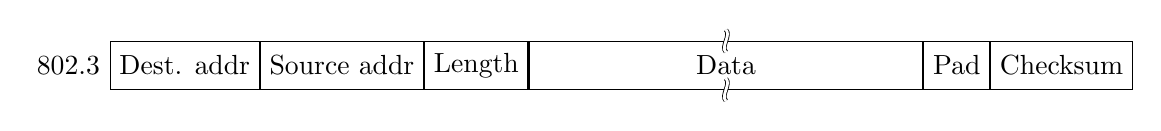
\begin{tikzpicture}[start chain, node distance=0pt]
  \label{page:inter:8023_header}
  \node [on chain] {802.3};
  \begin{scope}[every node/.style={on chain, draw, minimum height=4ex}]
    \node {Dest. addr};
    \node {Source  addr};
    \node {Length};
    \node [minimum width=5cm] (data) {Data};

    \variableLength{data}

    \node {Pad};
    \node {Checksum}; 
  \end{scope}
  
\end{tikzpicture}



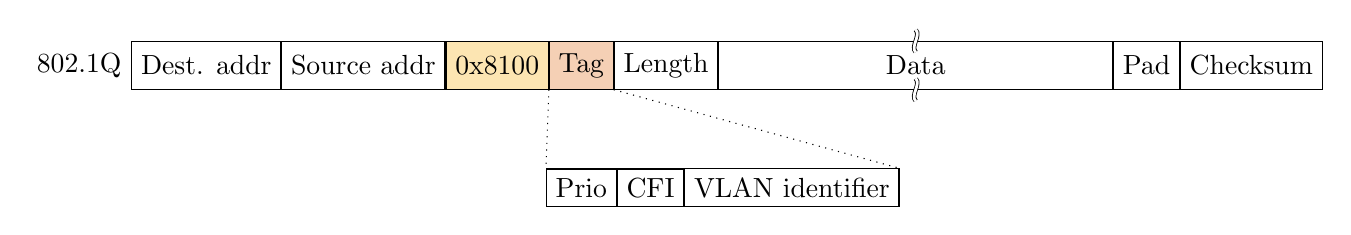
\begin{tikzpicture}[start chain=1, start chain=2, node distance=0pt]
  \label{page:inter:8021q_header}
  \node [on chain=1] {802.1Q};
  \begin{scope}[every node/.style={on chain=1, draw, minimum height=4ex}]
    \node {Dest. addr};
    \node {Source  addr};
    \node [fill=hpiyellow!30] (length) {0x8100};
    \node [fill=hpiorange!30] (tag) {Tag};
    \node {Length}; 
    \node [minimum width=5cm] (data) {Data};

    \variableLength{data}
    
    \node {Pad};
    \node {Checksum}; 
  \end{scope}

  \begin{scope}[every node/.style={draw}, node distance=0pt]
    \node [below=1cm of tag] (prio) {Prio}; 
    \node [right= of prio] (cfi) {CFI};
    \node [right=of cfi] (vlanid){VLAN identifier}; 
  \end{scope} 

  \draw [dotted] (tag.south west) -- (prio.north west) (tag.south east) -- (vlanid.north east); 
  
\end{tikzpicture}


\begin{tikzpicture}
  \label{page:inter:spanning_tree:network}

%   \node 
\end{tikzpicture}


\end{document}
